\chapter{Evaluation}

\section{Environment}

All the code has been run on the \enquote{Astral} high performance computer of Cranfield's university. The operating system is SUSE Linux Enterprise Server 11 (64 bits architecture), with a Linux 3 kernel.

The system is separated in login nodes and compute nodes. There are two \enquote{front-end} login nodes and they contain two Intel E5-2660 (Sandy Bridge - 8 cores) CPUs giving 16 CPU cores and have a total of 192 GB of shared memory. The login nodes enable the user to connect to the system and compile one's program. There are 80 compute nodes, each node having two Intel E5-2660 (Sandy Bridge - 8 cores) CPUs. This is giving a total of 1280 available cores. Each compute node have at least accessed to 64 GB shared memory. Nodes are connected with Infiniband\TM low-latency interconnect.

\section{Segmentation metrics}

To measure the precision of the localization / segmentation algorithm, we use the metrics as defined in \cite{pascalVoc2012} \footnote{Information on the evaluation system can be found at  \url{http://host.robots.ox.ac.uk/pascal/VOC/voc2012/devkit_doc.pdf}}.

To be considered a correct detection, the \textbf{Intersection over Union} $IoU$ between the predicted bounding box $B_p$ and ground truth bounding box $B_{gt}$ must exceed 50\% by the formula:

$$IoU = \frac{area(B_p \cap B_{gt})}{area(B_p \cup B_{gt})}$$

To simplify the calculation, this formula can be rewritten as:

$$IoU = \frac{area(B_p \cap B_{gt})}{area(B_p) + area(B_{gt}) - area(B_p \cap B_{gt})} $$

Using this metric, we can compute the precision $P$, the recall $R$ and the accuracy $A$ given by:

$$ P =  \frac{T_p}{T_p + F_p}$$
$$ R =  \frac{T_p}{T_p + F_n}$$
$$ A = \frac{T_p}{T_p + F_n + F_p} $$

with:
\begin{itemize}
   \item $T_p$ the number of true positives (the bounding boxes correctly localized)
   \item $F_p$ the number of false positives (the predicted bounding boxes incorrectly localized)
   \item $F_n$ the number of false negative (the ground truth bounding boxes not localized)
\end{itemize}

Note that given the convention from \cite{pascalVoc2012}, if more than one predicted bounding box overlaps the same ground truth bounding box, only one will be considered as $T_P$, the rest will be $F_P$s.

\section{Cross validation}

Cross validation is a technique used to assert the generalization to a new dataset of the different metrics used. 

A common type of cross validation is the k-fold cross validation. In this method, the  original sample is randomly split into $k$ partitions of equal sized. Of these generated subsamples, a single split is used for test set, the remaining are used as training data.
This last task is repeated $k$ times, each of the k partitions being used only once for testing. The $k$ results can then be averaged to produce a single estimation. 

The advantage of this method over repeated random sub-sampling is that all observations are used for both training and validation, and each observation is used for validation exactly once. 

10-fold cross-validation were used for all the presented results (the most common fold value that maximises the training set size).

\section{Results}

First, the localization and classification processes were run independantly (using the ground truth bounding box for classification).

\subsection{Food localisation}

\begin{table}
    \centering
    \renewcommand{\arraystretch}{1.2}
    \begin{tabular}{|c | c c|} 
        \hline
        Metric (average) & My method & DCNN from \cite{Bolanos2016} \\
        \hline
        Accuracy & \textbf{73 \%} & 60 \% \\ 
        \hline
        Recall &  \textbf{74 \%} & 80 \% \\
        \hline
        Precision &  \textbf{79 \%} & 70 \% \\
        \hline
    \end{tabular}
    \caption{Average localisation accuracy result for UEC FOOD 256}
\end{table}

In \cite{Bolanos2016}, the authors use fine-tuned pre-trained Deep Neural Network and obtain around

\subsection{Classification}

\begin{table}
    \centering
    \renewcommand{\arraystretch}{1.2}
    \begin{tabulary}{\textwidth}{| c | C|}
        \hline
        Method & Average accuracy \\
        \hline
        CNN as descriptor + RF & \textbf{40 \%} \\ 
        \hline
        BoW (1000 words)+ SVM with $\chi^2$ & 10 \% \\ % made up!
        \hline
        LBP + color historams and moments + Decision tree & 5 \% \\ 
        \hline
        LBP + color historams and moments + SVM & 11 \% \\ % made up!
        \hline
        LBP + color historams and moments + RF & 16 \% \\ % improved!
        \hline
        DCNN from \cite{Bolanos2016} & 63 \%\\
        \hline 
        DCNN from \cite{Yanai2015} & 67 \%\\
        \hline 
    \end{tabulary}
    \caption{Average classification accuracy result for UEC FOOD 256}
\end{table}

In \cite{Bolanos2016}, the authors use fine-tuned pre-trained Deep Neural Network and obtain 63 \% accuracyon UEC FOOD-256.

In \cite{Yanai2015}, the authors use fine-tuned pre-trained Deep Neural Network and obtain 67 \% accuracyon UEC FOOD-256.


\subsection{Segmentation followed by classification}

Using the segmentation and classification method with the highest accuracy, i.e. CNN Segmenter + CNN feature descriptor + RF classifier

\begin{table}
    \centering
    \renewcommand{\arraystretch}{1.2}
    \begin{tabulary}{\textwidth}{| c | C C|}
        \hline
        Process & My method & DCNN from \cite{Bolanos2016} \\
        \hline
        Overall & \textbf{28 \%} & 37 \% \\ 
        \hline
        Localisation &  \textbf{74 \%} & 60 \% \\
        \hline
        Classification &  \textbf{38 \%} & 60 \% \\
        \hline
    \end{tabulary}
    \caption{Average accuracy result for UEC FOOD 256}
\end{table}

\begin{figure}
    \centering
    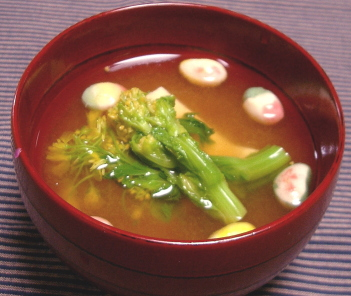
\includegraphics[height=2.5cm, width=2.5cm]{img/top_miso_soup.jpg}
    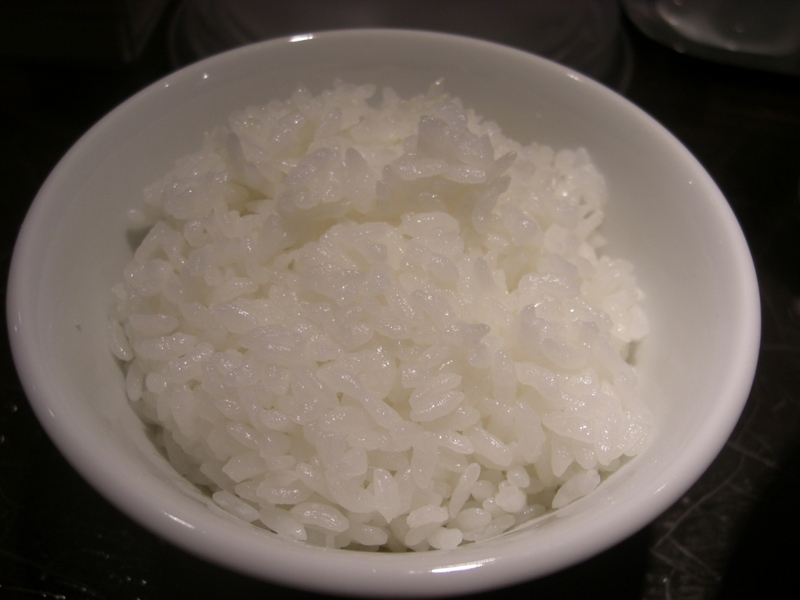
\includegraphics[height=2.5cm, width=2.5cm]{img/top_rice.jpg}
    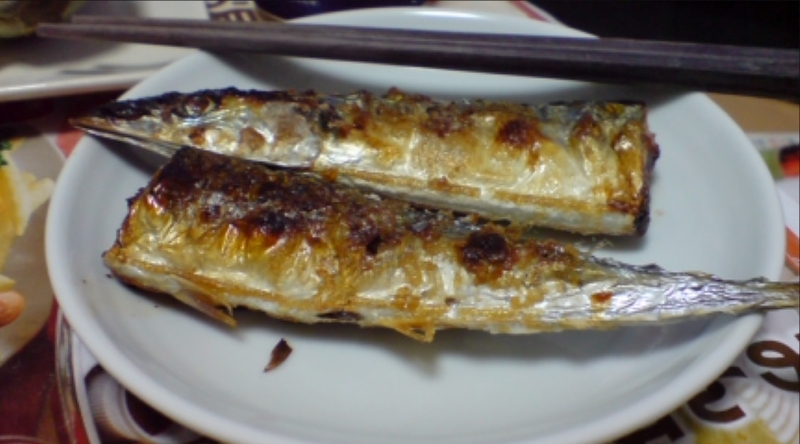
\includegraphics[height=2.5cm, width=2.5cm]{img/top_grilled_pacific_saury.jpg}
    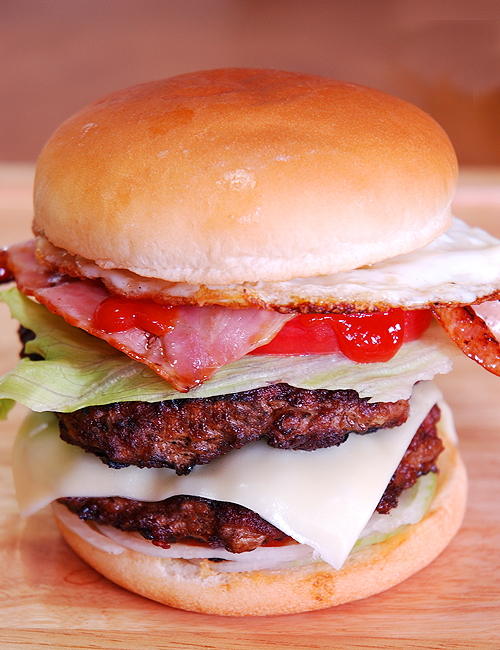
\includegraphics[height=2.5cm, width=2.5cm]{img/top_hamburger.jpg}
    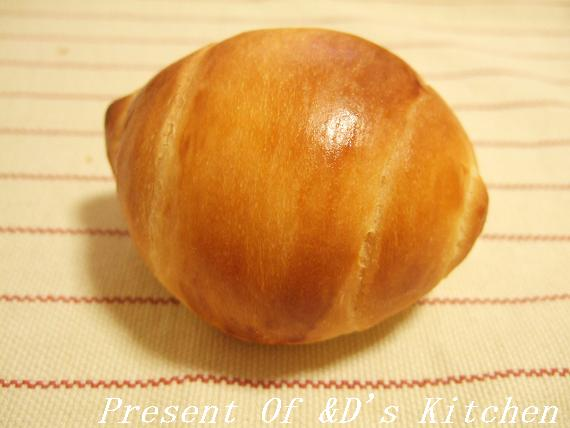
\includegraphics[height=2.5cm, width=2.5cm]{img/top_roll_bread.jpg}
    \caption[Top 5 accuracy classes]{Top 5 accuracy classes with (from the left to the right, starting from the highest accuracy) miso soup (98 \%), rice (95 \%), grilles pacific saury (94 \%), hamburger (93 \%), roll bread (90 \%)}
    \label{fig:top_5}
\end{figure}

14 roll bread 0.905660291919
17 hamburger 0.936073016618
49 grilled pacific saury 0.941860410357
1 rice 0.952117846186
36 miso soup 0.974164118934

\begin{figure}
    \centering
    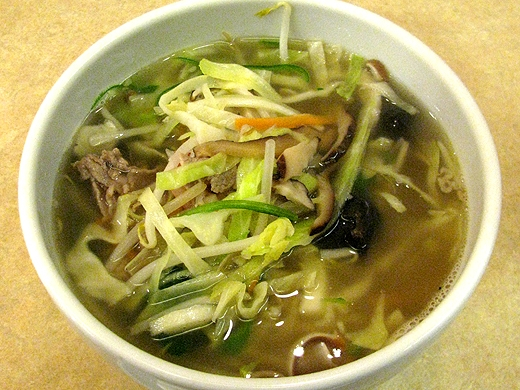
\includegraphics[height=2.5cm, width=2.5cm]{img/least_tanmen.jpg}
    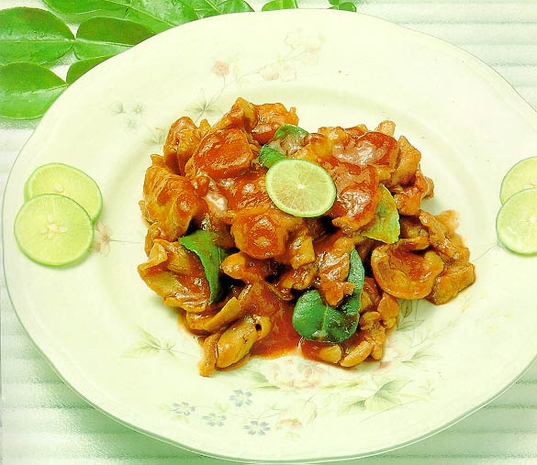
\includegraphics[height=2.5cm, width=2.5cm]{img/least_pork_with_lemon.jpg}
    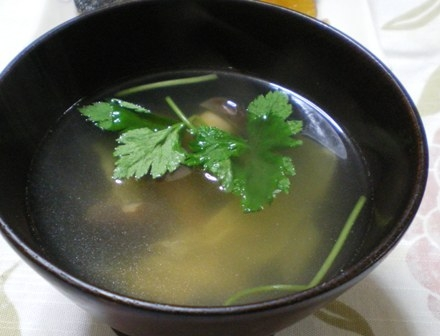
\includegraphics[height=2.5cm, width=2.5cm]{img/least_clear_soup.jpg}
    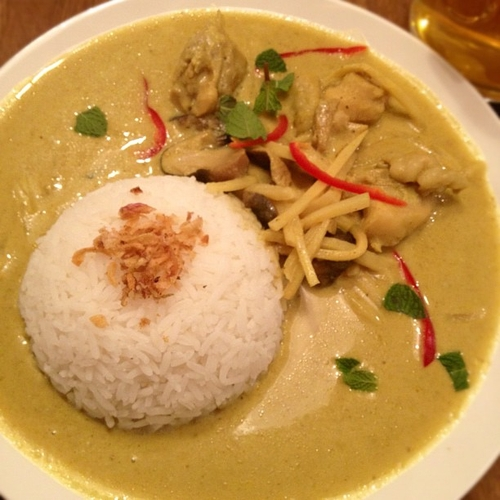
\includegraphics[height=2.5cm, width=2.5cm]{img/least_yellow_curry.jpg}
    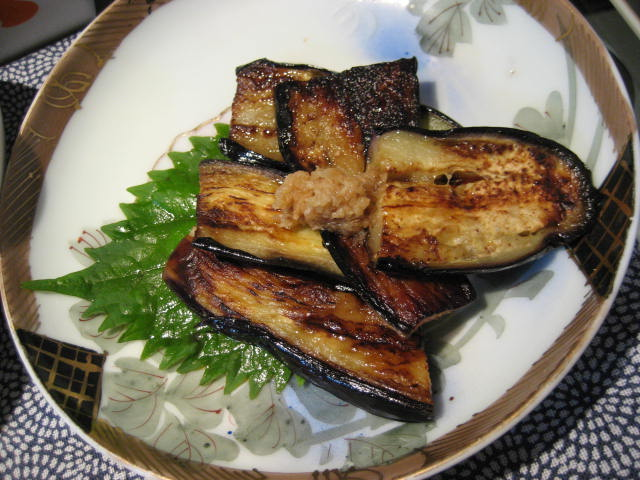
\includegraphics[height=2.5cm, width=2.5cm]{img/least_grilled_eggplant.jpg}
    \caption[Least 5 accuracy classes]{Least 5 accuracy classes with (from the left to the right, starting from the lowest accuracy) tanmen (0 \%), Pork with lemon (0 \%), clear soup (1 \%), yellow curry (1 \%), grilles eggplant (1 \%)}
    \label{fig:least_5}
\end{figure}

111 tanmen 0.0
193 Pork with lemon 0.0
135 clear soup 0.00952380861678
113 yellow curry 0.0104166655816
33 grilled eggplant 0.0105263146814

134 35 clear soup || miso soup 0.838095158277
88 35 Japanese tofu and vegetable chowder || miso soup 0.754716909932
124 35 zoni || miso soup 0.727272661157
156 35 oshiruko or red bean soup || miso soup 0.660194110661
82 5 cutlet curry || beef curry 0.658914677604
89 35 pork miso soup || miso soup 0.605504531605
7 8 chicken rice || fried rice 0.460674105542
23 22 beef noodle || ramen noodle 0.438596452755
238 11 kaya toast || toast 0.43434339047
135 35 yudofu || miso soup 0.431192620992


\cite{Bolanos2016} : accuracy 36.84 \%, 54.44 \% precision, Recall 50.86 \%

My classification is slightly less accurate as the bounding box as not as precise as the ground truth.

\begin{table}
    \centering
    \renewcommand{\arraystretch}{1.2}
    \begin{tabulary}{\textwidth}{| C | C c c|} 
        \hline
        Process & My method & DCNN from \cite{Shimoda2015} & DCNN from  \cite{Kawano2014} \\
        \hline
        Overall & \textbf{33 \%} & - & - \\ 
        \hline
        Localisation &  \textbf{67 \%} & 60 \% & - \\
        \hline
        Classification &  \textbf{50 \%} & -  & 72 \% \\
        \hline
    \end{tabulary}
    \caption{Average accuracy result for UEC FOOD 100}
\end{table}
